\chapter{Extensibility Guide}\label{chapter:extensibility}

This document discusses an implementation of a custom data acquirer (Section~\ref{section:custom_da}) and a custom data analyser (Section \ref{section:custom_ds}). Each section introduces concrete contract that has to be followed (see Section~\ref{section:extensibility}). When each acquirer or analyser is registered, it can be used during a new job configuration (see Figure~\ref{job-fe})

\begin{figure}[H]\label{job-fe}
\centering
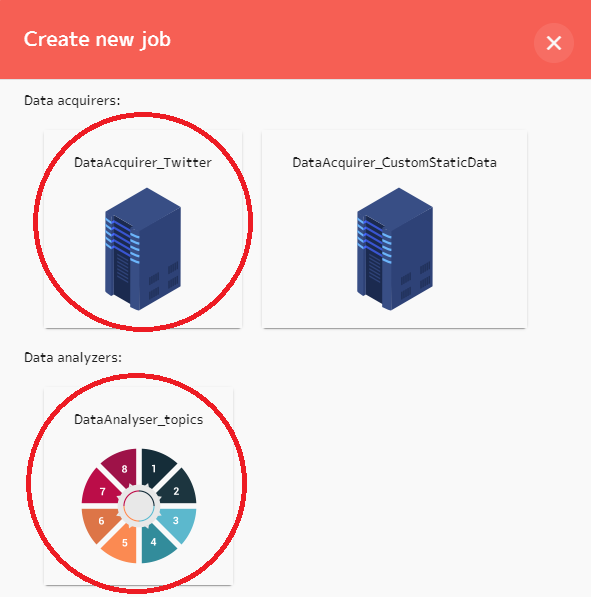
\includegraphics[width=0.7\textwidth]{diagrams/fe-job.png}
\caption{Screenshot of New Job form on Socneto front end. It shows all properly registered components}
\label{figure:monitoring-diagram}
\end{figure}

\section{Data Acquirer - QuoteLoader}\label{section:custom_da}

QuoteLoader loads data from a free API \url{http://quotes.rest/qod.json} returning random quotes.

\subsection{Contract}

\paragraph{Registration}

QuoteLoader sends registration request to the the topic\newline %\texttt{job\_management.registration.request}. \\ The registration request looks as follows:
\texttt{job\_management.registration.request}

\begin{lstlisting}[language=json,firstnumber=1]
{
  "componentId": "quoteLoaderDataAcquirer",
  "componentType": "DATA_ACQUIRER",
  "updateChannelName": "job_management.job_configuration.quoteLoaderDataAcquirer"
  }
}
\end{lstlisting}

Note that the \texttt{inputChannelName} is not present since QuoteLoader is data acquirer and does not have an input.

\paragraph{Starting the job}

QuoteLoader starts listening on a topic \newline
\texttt{job\_management.job\_configuration.quoteLoaderDataAcquirer}
 \\for a job like this:

\begin{lstlisting}[language=json,firstnumber=1]
{
    "jobId": "11d46859-3569-4bb1-9ec0-20eeac6ce132",
    "command": Start,
    "attributes":{},
    "outputChannelNames": [
        "job_management.component_data_input.storage_db",
        "job_management.component_data_input.some_analyser"]
}
\end{lstlisting}

Once the job notification arrives, QuoteLoader starts sending GET HTTP requests to \url{http://quotes.rest/qod.json}. QuoteLoader must remain listening to the topic while processing the newly arrived job. The endpoint returns JSON with the quote that looks like this (truncated for clarity):

\begin{lstlisting}[language=json,firstnumber=1]
{
    "quote": "You make a living by what you earn; you make a life by what you give.",
    "author": "Winston Churchill",
    "language": "en",
    "date": "2020-02-29",
    "id": "XZiOy4u9_g4Zmt7EdyxSIgeF"
}
\end{lstlisting}

The quote is then transformed into a post message and sent to both output channels \texttt{"job\_management.component\_data\_input.storage\_db"} and\newline \texttt{       "job\_management.component\_data\_input.some\_analyser"}.\\The post message looks like this:

\begin{lstlisting}[language=json,firstnumber=1]
{
  "id" : <new random uuid>,
  "jobId" : "11d46859-3569-4bb1-9ec0-20eeac6ce132", // from job notification
  "originalId" : "XZiOy4u9_g4Zmt7EdyxSIgeF", //quote id
  "text" : "You make a living by what you earn; you make a life by what you give.",
  "authorId" : "Winston Churchill",
  "language" : "en",
  "datetime" : "2020-02-29"
}
\end{lstlisting}
       
\paragraph{Stopping the job}

A stop job notification comes from the same topic as the start job notification. QuoteLoader listens on a topic \newline \texttt{job\_management.job\_configuration.quoteLoaderDataAcquirer} for a job like this:

\begin{lstlisting}[language=json,firstnumber=1]
{
    "jobId": "11d46859-3569-4bb1-9ec0-20eeac6ce132",
    "command": Stop
}
\end{lstlisting}

Quote loader stops the job while still listening on a the topic for new jobs.

\section{Data Analyser - Hashtags}\label{section:custom_ds}

This section describes on a real implementation, how can be a new analyser added to  Socneto.

\subsection{Contracts}

Hashtag analyser is implemented to simulate the easy extensibility of analysers. This component has a simple goal: compute frequencies of hashtags in posts.

\paragraph{Registration}

The analyser sends a registration request to the the topic \newline \texttt{job\_management.registration.request}. \\The registration request looks as follows:

\begin{lstlisting}[language=json,firstnumber=1]
{
  "componentId": "HashTags",
  "componentType": "DATA_ANALYSER",
  "inputChannelName": "job_management.component_data_input.HASH_TAG",
"updateChannelName": "job_management.job_configuration.HASH_TAG"
  }
}
\end{lstlisting}

\paragraph{Starting the Job}

The Hashtag analyser is stateless, so it does not need update messages. All posts are always analysed and sent to storage on a topic:\\ \texttt{job\_management.component\_data\_analyzed\_input.storage\_db}\\

\paragraph{Analysing posts}

When the post message is received, the module creates a frequency map of found hashtags and sends the analysis message to the storage
\\

\noindent
\textbf{Example post message:}


\begin{lstlisting}[language=json,firstnumber=1]
{
  "id" :"9e36b903-7f1b-43dd-b4f8-f64a8f95245d",
  "jobId" : "11d46859-3569-4bb1-9ec0-20eeac6ce132",
  "originalId" : "XZiOy888_g4Zmt7EdyxSazc",
  "text" : "#czech_castle #top09 Kalousek na hrad.",
  "authorId" : "Andrej",
  "language" : "cz",
  "datetime" : "2020-02-29"
}
\end{lstlisting}

\noindent
\textbf{Example analysis:}

\begin{lstlisting}[language=json,firstnumber=1]
{
  "postId": "9e36b903-7f1b-43dd-b4f8-f64a8f95245d",
  "jobId": "11d46859-3569-4bb1-9ec0-20eeac6ce132",
  "componentId": HashTags,
  "results": {
    "valueName": {
        "numberValue": null
        "textValue": null
        "numberListValue": null
        "textListValue": null
        "numberMapValue": {
                "czech_castle": 1,
                "top09": 1
        },
        "textMapValue": null
    }
  }
}
\end{lstlisting}
       
\paragraph{Stopping the Job}

Because this analyser is stateless, it does not need to work with the stop job procedure.

\subsection{Java Skeleton}\label{section:custom_ds}

The Hashtag analyser is implemented on  top of our prepared Java Spring skeleton for an easy analyser implementation. This implementation is stored in \textit{generic\_analyser} folder. There is a list of steps, that must be followed to integrate a new analyser into the platform from this skeleton.

\begin{itemize}
  
  \item A new analyser must have configured these properties \textit{in application.proper\-ties}:
  
  \begin{itemize}
  \item Unique component id
	\begin{itemize}
        \item property: \texttt{component.config.componentId}
    \end{itemize}
  
  \item Topic for new posts
    \begin{itemize}
	    \item property: \texttt{component.config.topicInput}
        \item conventionally with prefix: \texttt{job\_management.component\_data\_in\-put}
    \end{itemize}
  
  \item Topic for job updates
    \begin{itemize}
	    \item property: \texttt{component.config.topicUpdate}
        \item conventionally with prefix: \texttt{job\_management.job\_configuration}
   \end{itemize}
  
  \item Spring profile
    \begin{itemize}
	    \item property: \texttt{spring.profiles.active}
   \end{itemize}
  \item Output format (described in Section \ref{subsubsection:registration_analyser})
  
  \end{itemize}
  
  \item Orchestration is prepared and the only one thing is to implement the \texttt{cz.cuni.mff.socneto.storage.analyzer.Analyzer} interface. There are two methods, that must be overridden:
  \begin{itemize}
	    \item \texttt{Map$<$String, String$>$ getFormat()}
	    \begin{itemize}
	        \item an output format for registration message (the structure is described in Section \ref{subsubsection:registration_analyser})
        \end{itemize}
	    \item \texttt{$<$MapString, AnalysisResult$>$ analyze(String text)}
	    \begin{itemize}
	        \item input: a text to analyse
	        \item output: a result in the same format as the format returned in the method \textit{getFormat}
        \end{itemize}
   \end{itemize}
\end{itemize}

This approach should help an expert users of Socneto to implement a new analyser with reusing common and required parts of all analysers.
